% Options for packages loaded elsewhere
\PassOptionsToPackage{unicode}{hyperref}
\PassOptionsToPackage{hyphens}{url}
\PassOptionsToPackage{dvipsnames,svgnames,x11names}{xcolor}
%
\documentclass[
  letterpaper,
  DIV=11,
  numbers=noendperiod]{scrartcl}

\usepackage{amsmath,amssymb}
\usepackage{iftex}
\ifPDFTeX
  \usepackage[T1]{fontenc}
  \usepackage[utf8]{inputenc}
  \usepackage{textcomp} % provide euro and other symbols
\else % if luatex or xetex
  \usepackage{unicode-math}
  \defaultfontfeatures{Scale=MatchLowercase}
  \defaultfontfeatures[\rmfamily]{Ligatures=TeX,Scale=1}
\fi
\usepackage{lmodern}
\ifPDFTeX\else  
    % xetex/luatex font selection
\fi
% Use upquote if available, for straight quotes in verbatim environments
\IfFileExists{upquote.sty}{\usepackage{upquote}}{}
\IfFileExists{microtype.sty}{% use microtype if available
  \usepackage[]{microtype}
  \UseMicrotypeSet[protrusion]{basicmath} % disable protrusion for tt fonts
}{}
\makeatletter
\@ifundefined{KOMAClassName}{% if non-KOMA class
  \IfFileExists{parskip.sty}{%
    \usepackage{parskip}
  }{% else
    \setlength{\parindent}{0pt}
    \setlength{\parskip}{6pt plus 2pt minus 1pt}}
}{% if KOMA class
  \KOMAoptions{parskip=half}}
\makeatother
\usepackage{xcolor}
\setlength{\emergencystretch}{3em} % prevent overfull lines
\setcounter{secnumdepth}{-\maxdimen} % remove section numbering
% Make \paragraph and \subparagraph free-standing
\makeatletter
\ifx\paragraph\undefined\else
  \let\oldparagraph\paragraph
  \renewcommand{\paragraph}{
    \@ifstar
      \xxxParagraphStar
      \xxxParagraphNoStar
  }
  \newcommand{\xxxParagraphStar}[1]{\oldparagraph*{#1}\mbox{}}
  \newcommand{\xxxParagraphNoStar}[1]{\oldparagraph{#1}\mbox{}}
\fi
\ifx\subparagraph\undefined\else
  \let\oldsubparagraph\subparagraph
  \renewcommand{\subparagraph}{
    \@ifstar
      \xxxSubParagraphStar
      \xxxSubParagraphNoStar
  }
  \newcommand{\xxxSubParagraphStar}[1]{\oldsubparagraph*{#1}\mbox{}}
  \newcommand{\xxxSubParagraphNoStar}[1]{\oldsubparagraph{#1}\mbox{}}
\fi
\makeatother


\providecommand{\tightlist}{%
  \setlength{\itemsep}{0pt}\setlength{\parskip}{0pt}}\usepackage{longtable,booktabs,array}
\usepackage{calc} % for calculating minipage widths
% Correct order of tables after \paragraph or \subparagraph
\usepackage{etoolbox}
\makeatletter
\patchcmd\longtable{\par}{\if@noskipsec\mbox{}\fi\par}{}{}
\makeatother
% Allow footnotes in longtable head/foot
\IfFileExists{footnotehyper.sty}{\usepackage{footnotehyper}}{\usepackage{footnote}}
\makesavenoteenv{longtable}
\usepackage{graphicx}
\makeatletter
\def\maxwidth{\ifdim\Gin@nat@width>\linewidth\linewidth\else\Gin@nat@width\fi}
\def\maxheight{\ifdim\Gin@nat@height>\textheight\textheight\else\Gin@nat@height\fi}
\makeatother
% Scale images if necessary, so that they will not overflow the page
% margins by default, and it is still possible to overwrite the defaults
% using explicit options in \includegraphics[width, height, ...]{}
\setkeys{Gin}{width=\maxwidth,height=\maxheight,keepaspectratio}
% Set default figure placement to htbp
\makeatletter
\def\fps@figure{htbp}
\makeatother

\KOMAoption{captions}{tableheading}
\makeatletter
\@ifpackageloaded{caption}{}{\usepackage{caption}}
\AtBeginDocument{%
\ifdefined\contentsname
  \renewcommand*\contentsname{Table of contents}
\else
  \newcommand\contentsname{Table of contents}
\fi
\ifdefined\listfigurename
  \renewcommand*\listfigurename{List of Figures}
\else
  \newcommand\listfigurename{List of Figures}
\fi
\ifdefined\listtablename
  \renewcommand*\listtablename{List of Tables}
\else
  \newcommand\listtablename{List of Tables}
\fi
\ifdefined\figurename
  \renewcommand*\figurename{Figure}
\else
  \newcommand\figurename{Figure}
\fi
\ifdefined\tablename
  \renewcommand*\tablename{Table}
\else
  \newcommand\tablename{Table}
\fi
}
\@ifpackageloaded{float}{}{\usepackage{float}}
\floatstyle{ruled}
\@ifundefined{c@chapter}{\newfloat{codelisting}{h}{lop}}{\newfloat{codelisting}{h}{lop}[chapter]}
\floatname{codelisting}{Listing}
\newcommand*\listoflistings{\listof{codelisting}{List of Listings}}
\makeatother
\makeatletter
\makeatother
\makeatletter
\@ifpackageloaded{caption}{}{\usepackage{caption}}
\@ifpackageloaded{subcaption}{}{\usepackage{subcaption}}
\makeatother

\ifLuaTeX
  \usepackage{selnolig}  % disable illegal ligatures
\fi
\usepackage{bookmark}

\IfFileExists{xurl.sty}{\usepackage{xurl}}{} % add URL line breaks if available
\urlstyle{same} % disable monospaced font for URLs
\hypersetup{
  pdftitle={Workshop 1},
  pdfauthor={Aprendizaje Estadístico 2},
  colorlinks=true,
  linkcolor={blue},
  filecolor={Maroon},
  citecolor={Blue},
  urlcolor={Blue},
  pdfcreator={LaTeX via pandoc}}


\title{Workshop 1}
\author{Aprendizaje Estadístico 2}
\date{}

\begin{document}
\maketitle


Solve the next exercises using computational tools like R or Python, R
Mardown or Google Colab. Make a pdf report where you show the whole
procedure. Take into account that you have to be clear because it is
something to be assesed.

\subsection{Experiment Setup}\label{experiment-setup}

From exercise 1 to 5 consider the sample space of tossing a fair coin 3
times:

\[S=\{HHH,HHT,HTH,THH,HTT,THT,TTH,TTT\}\]

with each outcome having probability \(1/8\).

\begin{enumerate}
\def\labelenumi{\arabic{enumi}.}
\tightlist
\item
  Describe the next events:
\end{enumerate}

\(A:\) ``first toss is \(H\).'' \(B:\) ``second toss is \(H\).'' \(C:\)
``all tosses are \(H\).'' \(D:\) ``exactly one \(H\).''

\begin{enumerate}
\def\labelenumi{\arabic{enumi}.}
\setcounter{enumi}{1}
\item
  Check if \(A\) and \(B\) are independent. Are they mutually exclusive?
\item
  Check if \(C\) and \(D\) are independent. Are they mutually exclusive?
\item
  Prove: If two events \(E, F\) are mutually exclusive and both have
  positive probability, then they cannot be independent.
\item
  Take event \(G=\) ``first toss is head,'' \(G^C=\) ``first toss is
  tail.'' Show \(G\) and \(G^C\) are mutually exclusive and compute
  whether they are independent.
\item
  Compute \(P(Z \ge 1.96)\) for a standard normal
  \(Z \sim \mathcal N(0,1)\) and illustrate it by shading the right
  tail.
\end{enumerate}

Using pnorm(), compute \(P(Z \ge 1.96)\).

Make a plot of the standard normal density on \(x \in [-4,4]\) with the
right tail (\(x \ge 1.96\)) shaded.

\begin{enumerate}
\def\labelenumi{\arabic{enumi}.}
\setcounter{enumi}{6}
\tightlist
\item
  For \(Z \sim \mathcal N(0,1)\) compute:
\end{enumerate}

\begin{enumerate}
\def\labelenumi{(\alph{enumi})}
\item
  \(P(Z \le -1.5)\)
\item
  \(P(Z \ge 2.1)\)
\item
  \(P(|Z| \ge 2)\)
\item
  The central 95\% probability \(P(-z \le Z \le z)\) and the value of
  \(z\) such that this equals \(0.95\).
\end{enumerate}

\begin{enumerate}
\def\labelenumi{\arabic{enumi}.}
\setcounter{enumi}{7}
\item
  dd

  \begin{enumerate}
  \def\labelenumii{(\alph{enumii})}
  \item
    Find the 90th percentile of \(Z \sim \mathcal N(0,1)\), i.e.,
    compute \(z_{0.90}\) such that \(P(Z \le z_{0.90})=0.90\).
  \item
    Find \(z\) such that \(P(|Z| \le z)=0.90\).
  \item
    Suppose \(X \sim \mathcal N(\mu=100, \sigma=15)\). Compute the score
    threshold \(c\) for the top 5\%.
  \end{enumerate}
\item
  For \(Z \sim \mathcal N(0,1)\):
\end{enumerate}

\begin{enumerate}
\def\labelenumi{(\alph{enumi})}
\item
  Simulate \(N=100{,}000\) draws and estimate \(P(Z \ge 1.96)\)
  empirically.

\begin{verbatim}
[1] 5.229527
\end{verbatim}

  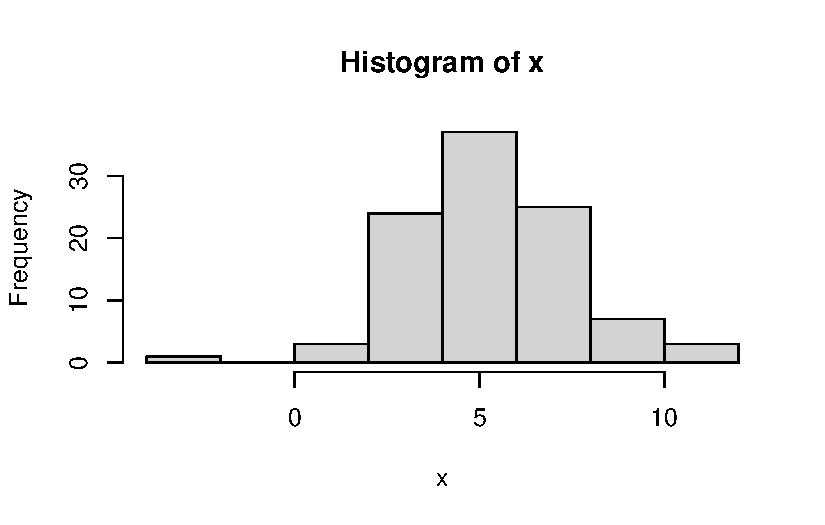
\includegraphics{WS1-APE2-a_files/figure-pdf/unnamed-chunk-15-1.pdf}
\item
  Compare with the exact value.
\item
  Plot a histogram with an overlaid theoretical density curve.
\end{enumerate}

\begin{enumerate}
\def\labelenumi{\arabic{enumi}.}
\setcounter{enumi}{9}
\tightlist
\item
  Let \(X \sim \mathcal N(\mu=70,\ \sigma=8)\). Compute:
\end{enumerate}

\begin{enumerate}
\def\labelenumi{(\alph{enumi})}
\item
  \(P(X \le 60)\)
\item
  \(P(65 \le X \le 85)\)
\item
  The 2.5th percentile of \(X\)
\end{enumerate}

Do each both directly and by standardizing to
\(Z=\dfrac{X-\mu}{\sigma}\).

\begin{enumerate}
\def\labelenumi{\arabic{enumi}.}
\setcounter{enumi}{10}
\item
  Generate \(N=200\) observations from
  \(\mathcal N(\mu = 5, \sigma^2=2^2)\), then:
\end{enumerate}

\begin{enumerate}
\def\labelenumi{(\alph{enumi})}
\item
  Plot histogram with density overlay.
\item
  Make a QQ‑plot to assess normality.
\end{enumerate}

\begin{enumerate}
\def\labelenumi{\arabic{enumi}.}
\setcounter{enumi}{11}
\item
  \begin{enumerate}
  \def\labelenumii{(\alph{enumii})}
  \item
    For \(Z \sim \mathcal N(0,1)\), compute \(z_\alpha\) such that
    \(P(|Z| \le z_\alpha) = 0.99\).
  \item
    For \(X \sim \mathcal N(\mu = 120, \sigma=10)\), find the symmetric
    90\% interval around the mean.
  \item
  \item
    Verify by simulation that about 90\% of draws fall in your interval
    from (b).
  \end{enumerate}
\end{enumerate}




\end{document}
